\clearpage
\setcounter{page}{1}
\maketitlesupplementary

\setcounter{section}{0}%
\renewcommand{\thesection}{\Alph{section}}



\noindent We organize the supplementary as follows: 

\begin{itemize}

    \item Section~\ref{sup:sec_corruption}: Corruption modes in AMOS
    \item Section~\ref{sup:qualitative}: Qualitative results
    \item Section~\ref{sup:ablations}: Ablation analysis
    \item Section~\ref{sup:compositional}: Compositional image retrieval
    \item Section~\ref{sup:gt-cond-img-ret}: Geo-temporal image retrieval analysis
    \item Section~\ref{sup:time-pred}: Time prediction analysis
    \item Section~\ref{sup:training-details}: Training details
    \item Section~\ref{sup:embedding}: Embedding space visualization

\end{itemize}


\section{Corruption modes in AMOS}
\label{sup:sec_corruption}

\setlength{\columnsep}{6pt}%
\begin{wrapfigure}[9]{r}{0.5\linewidth}
\vspace{-16pt}
  \centering
  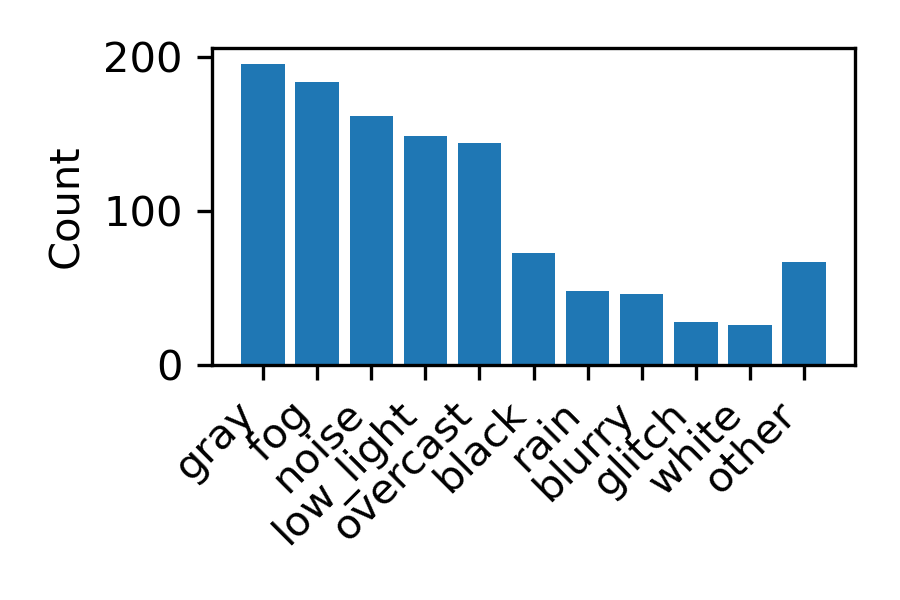
\includegraphics[width=\linewidth, trim=26 14 0 0, clip]{figures/low_quality_distribution.png}
    \vspace{-7mm}
    \captionsetup{font=small}
    \caption{\bf{Distribution of corruption modes in AMOS.}}
  \label{fig:corr-count}
\end{wrapfigure}

Figure~\ref{fig:corr-count} presents the distribution of corruption modes observed in the manually annotated samples from the original AMOS dataset. Complementary qualitative examples are shown in Figure~\ref{fig:corruptions}, highlighting the wide variability and visual characteristics of these corruptions. The observed artifacts stem from a combination of environmental conditions, sensor and hardware degradation, and network-related issues. As a result, the dataset cannot be reliably used in its raw form and requires substantial filtering prior to downstream applications.
We categorize these failure modes into four broad groups: (i) \textbf{Sensor or hardware failures}, including black frames, broken lenses, dead pixels, and “no feed” placeholders; (ii) \textbf{Environmental conditions}, such as fog, rain, overcast skies, or low-light nighttime scenes; (iii) \textbf{Imaging and compression artifacts}, including blur, flare, Gaussian noise, glitches, or unnatural color balance; and (iv) \textbf{Content or framing errors}, such as indoor captures, floor views, or non-visual placeholders (e.g., weather maps, static logos).
These corruptions can dominate the raw corpus, with many cameras producing long sequences of invalid or heavily degraded frames. To construct a reliable benchmark, we developed a semi-supervised filtering pipeline (Section~\ref{sec:data_curation}, Figure~\ref{fig:data_pipeline} in the main paper) that automatically detects and removes such samples while preserving geographic and temporal diversity. We show additional examples of images that were ultimately classified as high, medium and low-quality in Figure~\ref{fig:quality_examples}.

\begin{figure}[t]
\begin{center}
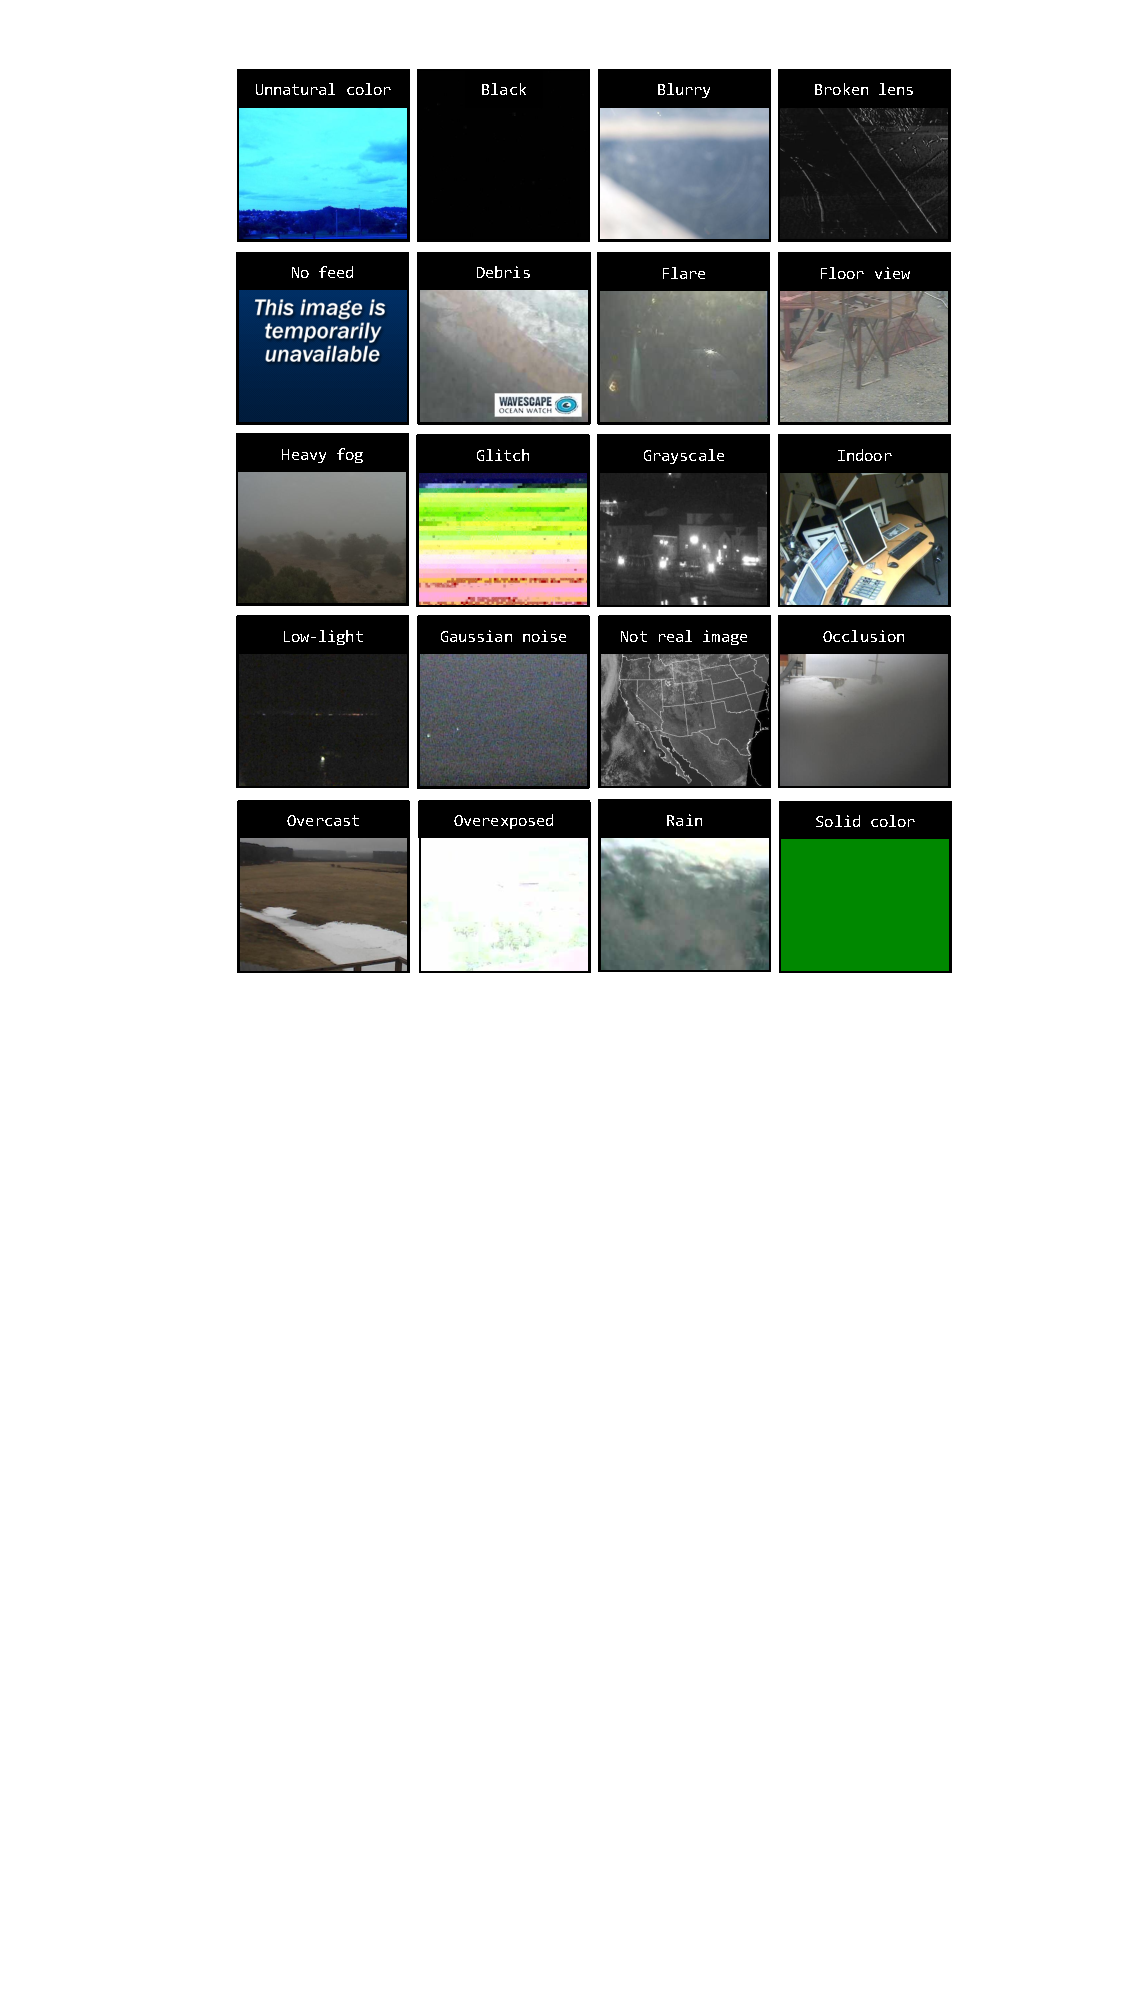
\includegraphics[width=0.95\linewidth]{figures/corruption_modes.pdf}
\end{center}
\vspace{-1em}
\caption{\textbf{Corruption modes in the AMOS dataset.}
Examples of typical failure modes in raw AMOS imagery, including sensor or hardware issues (black frames, dead pixels, broken lenses, ``no feed'' screens), challenging environmental conditions (fog, rain, nighttime), imaging and compression artifacts (blur, glare, noise, color shifts), and content or framing errors (indoor views, floor shots, overlays, or static graphics). 
These corruptions are frequent and often persistent over time, underscoring the need for the filtering pipeline described in Section~\ref{sec:data_curation}.}
\label{fig:corruptions}
\end{figure}

\begin{figure}[t]
\begin{center}
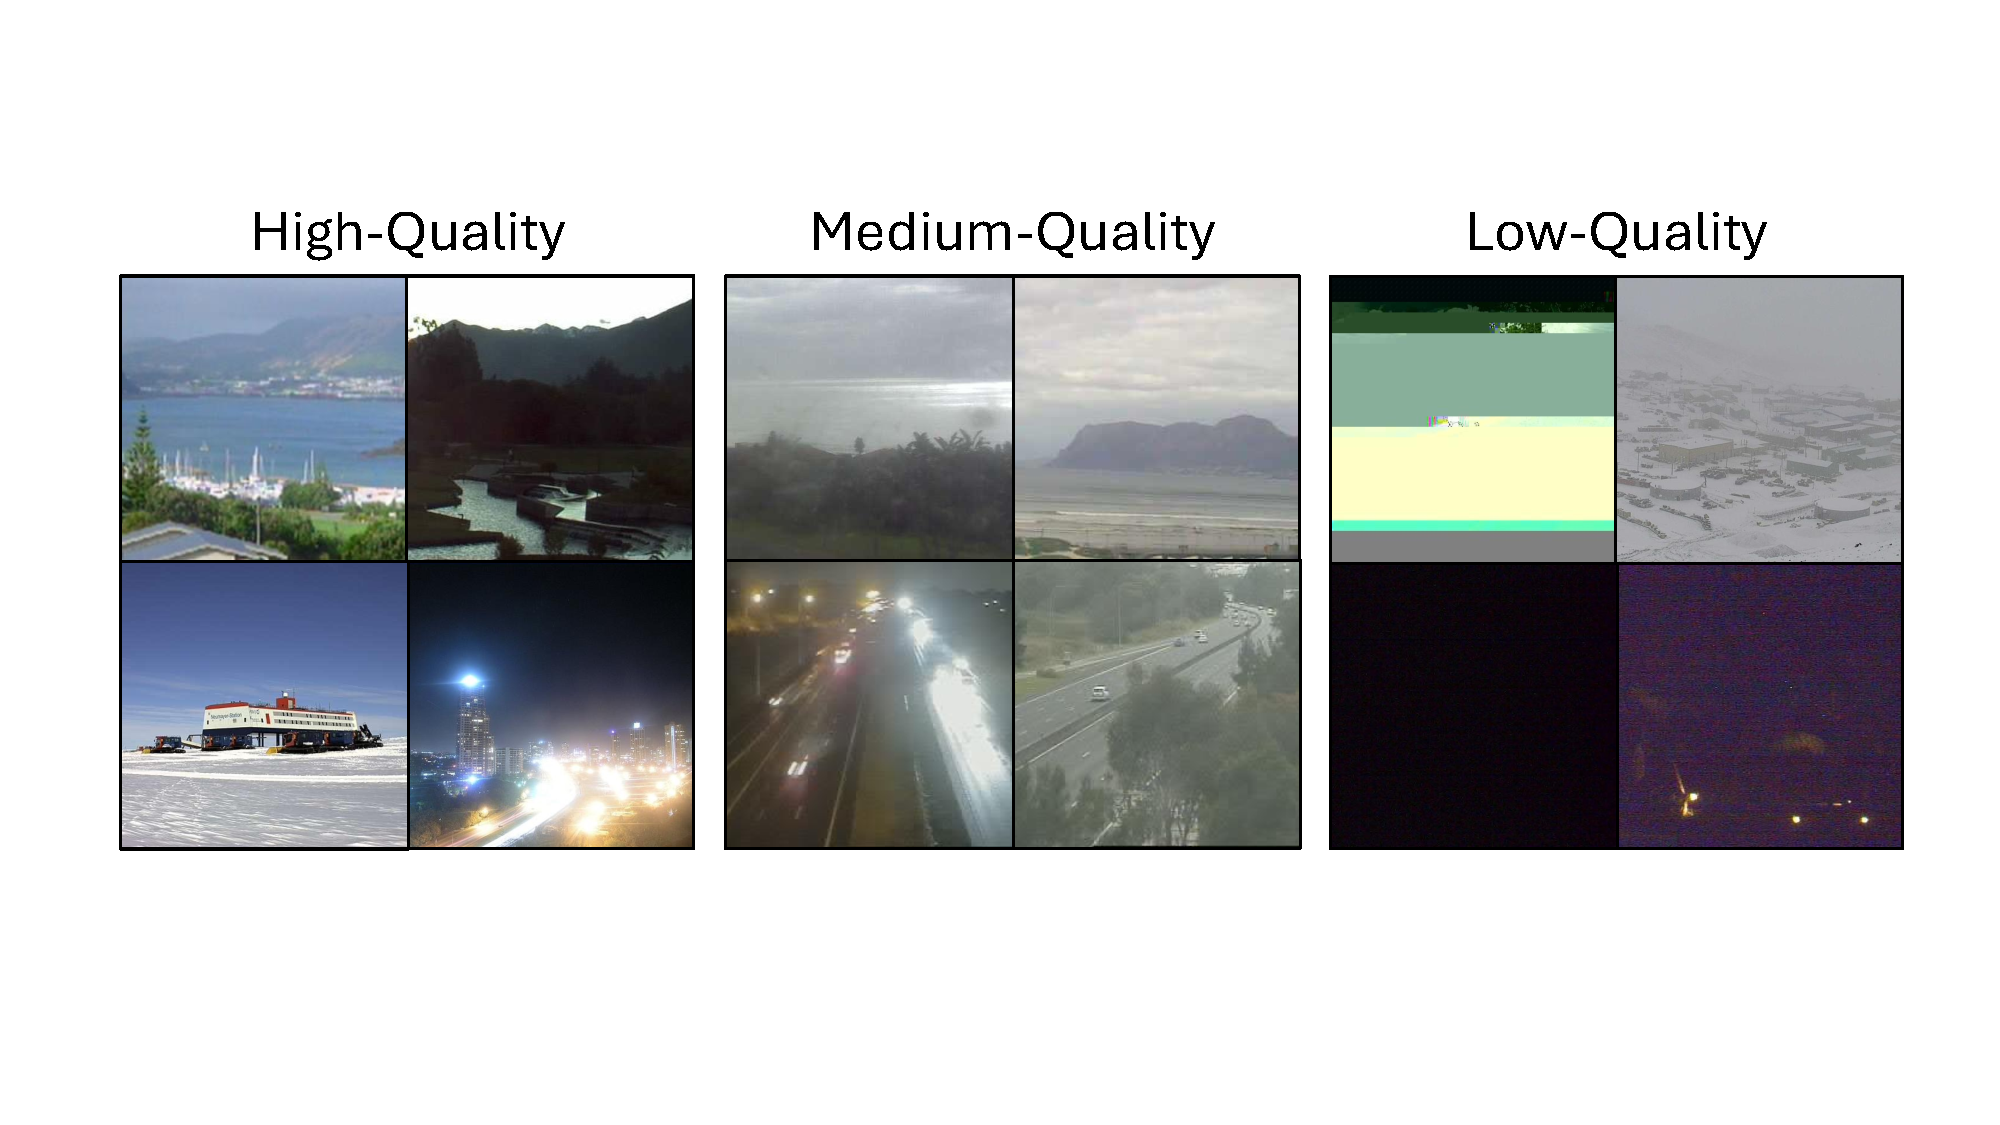
\includegraphics[width=0.98\linewidth]{figures/quality_examples.pdf}
\end{center}
\vspace{-1em}
\caption{Sample images that were classified as high, medium or low-quality by our semi-supervised data curation pipeline.}
\label{fig:quality_examples}
\end{figure}


\section{Qualitative results}
\label{sup:qualitative}

\noindent \textbf{Time prediction.} Figure~\ref{fig:time-pred-dist} illustrates how \tiger\ models time from a single image. For each query image, we compute cosine similarities between its visual embedding and a gallery of time embeddings, then aggregate the scores into 1-month (or 1-hour) bins and apply a softmax to obtain a probability distribution over time-of-year (ToY) or time-of-day (ToD). On the left, we show three queries captured around the same ToD (between 6--7 AM) but in different months (March, July, and August); the predicted distributions are defined over months and peak near the ground-truth ToY, with most mass concentrated in neighboring bins. On the right, the queries all come from January but at different hours; here the distributions are defined over hours and again peak near the ground-truth ToD. These results indicate that \tiger\ produces sharp, well-localized temporal distributions that accurately reflect both ToY and ToD.

\begin{figure*}
\begin{center}
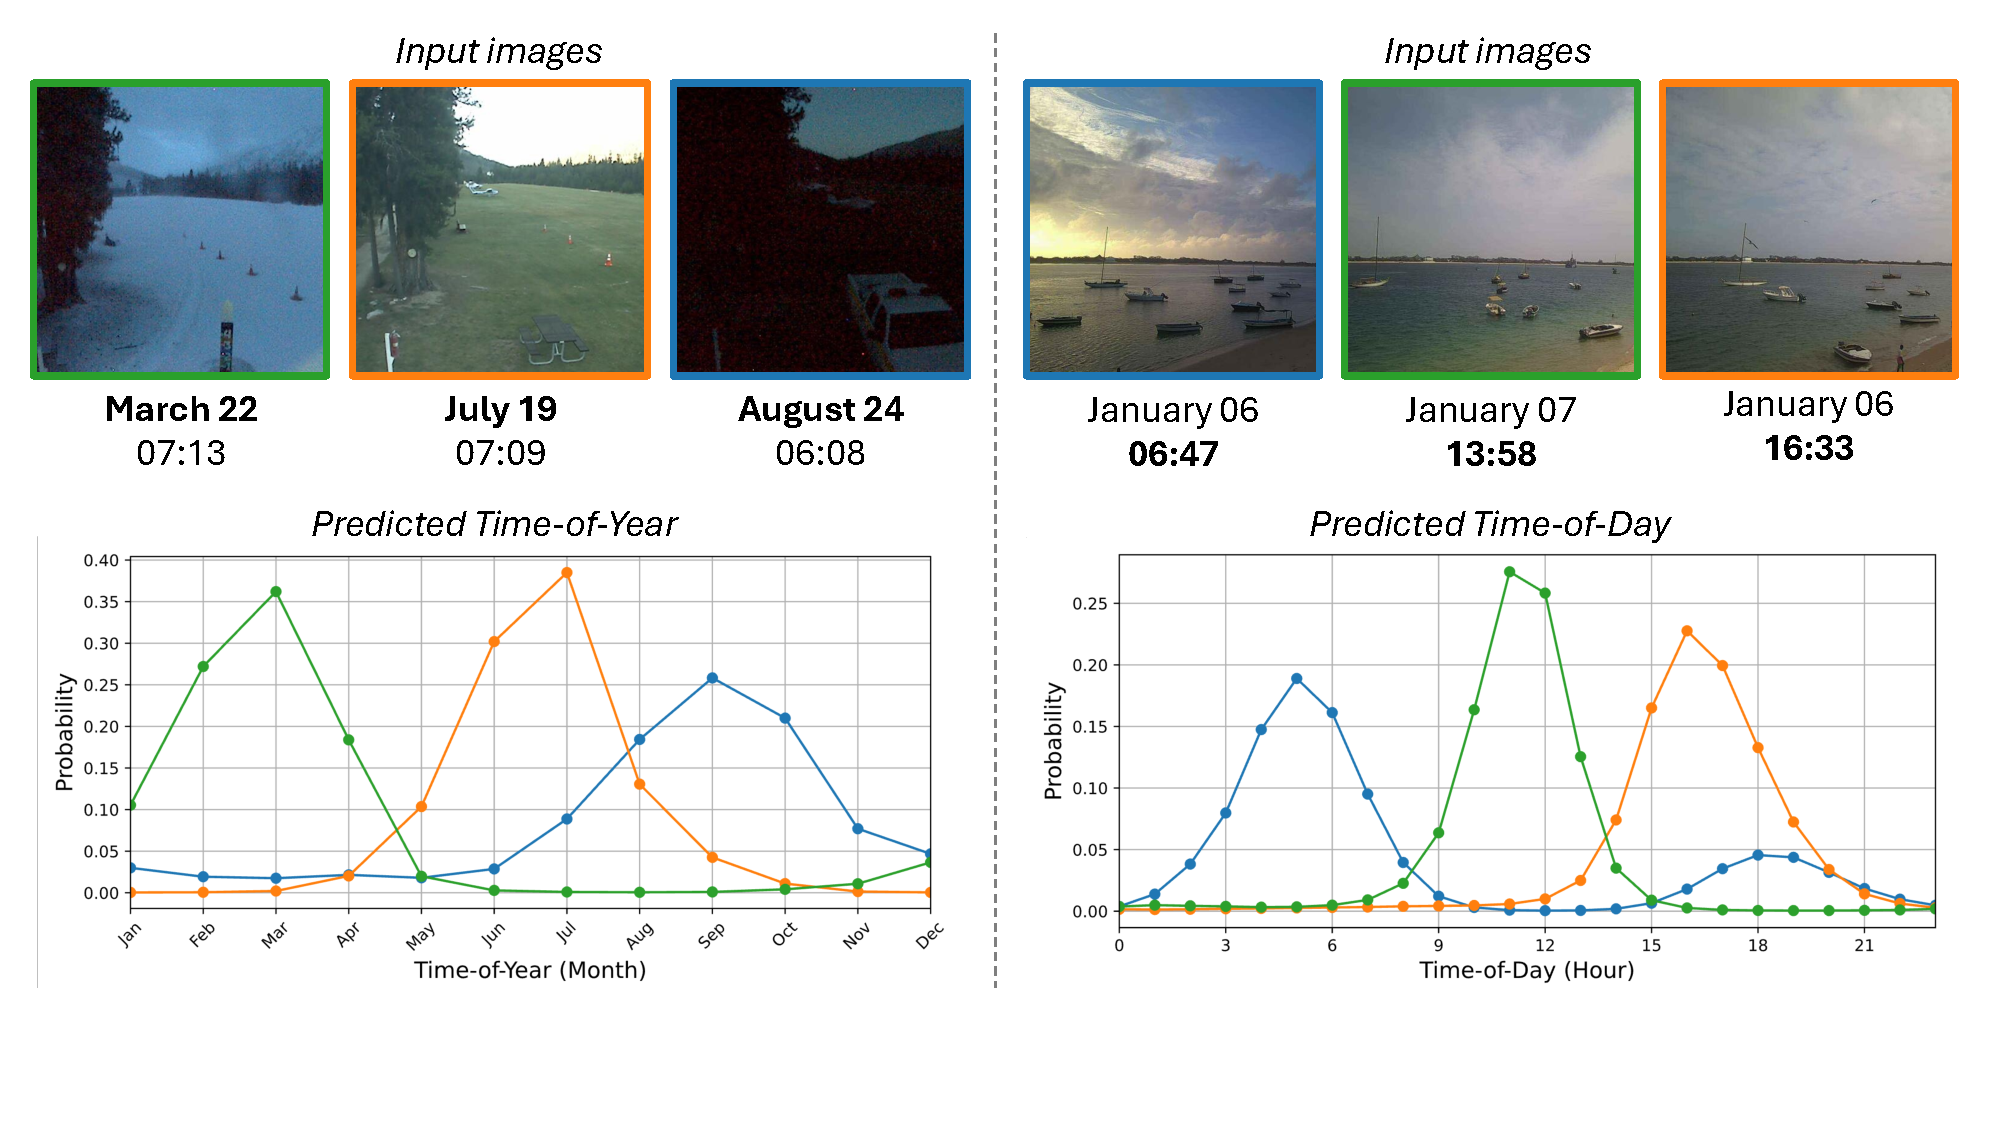
\includegraphics[width=0.9\linewidth]{figures/time_pred_dist.pdf}
\end{center}
\vspace{-1em}
\caption{\textbf{Time prediction probabilities}. For an input image $I^Q$, we compute cosine similarity between it's visual embedding $\bar{\textbf{v}}^Q$ and a gallery of time embeddings $\bar{\textbf{t}}^G$, sampled at 1-hour and 1-month intervals. The similarity vector is normalized using the softmax operator, resulting in a predicted time probability distribution.
\textbf{Left}: Comparison of the predicted time-of-year probabilities for images at roughly the same time-of-day, but different time-of-years. \textbf{Right}: Comparison of the predicted time-of-day probabilities for images at roughly the same time-of-year, but different time-of-days.}
\label{fig:time-pred-dist}
\end{figure*}

\noindent \textbf{Geo-localization.} Figure~\ref{fig:qual-geo} shows how \tiger\ localizes three CVT test images taken in geographically diverse regions. For each query image, we display the corresponding distribution of retrieved GPS candidates, highlighting both the predicted and ground-truth locations to illustrate the sharpness and accuracy of the model’s geo-localization.

\begin{figure}[h]
\begin{center}
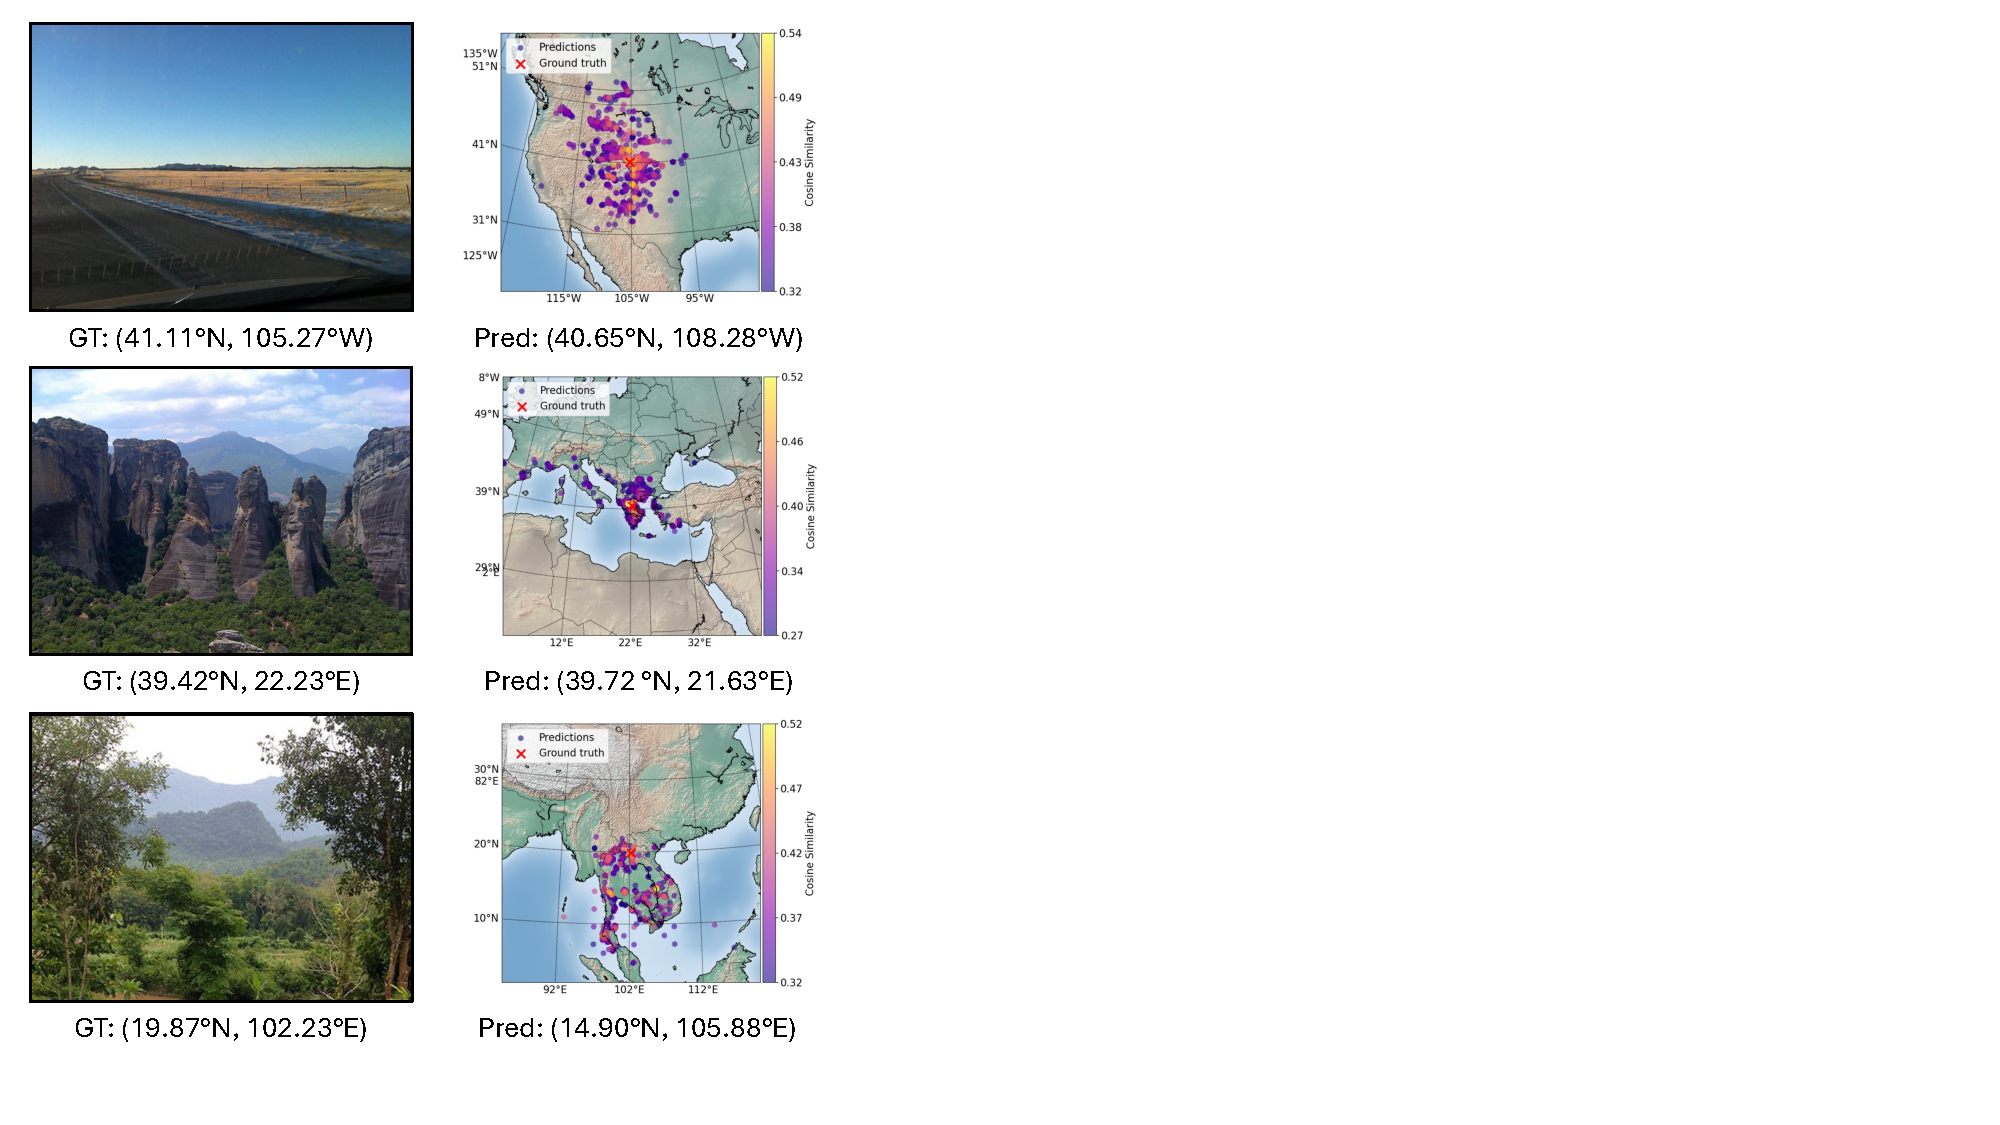
\includegraphics[width=0.9\linewidth]{figures/qual_geo.pdf}
\end{center}
\vspace{-1em}
\caption{\textbf{Qualitative geo-localization examples on CVT.} Each row shows a query image (left) annotated with its ground-truth GPS coordinate, and the corresponding map of retrieved locations (right). We plot the top-1k candidate GPS coordinates predicted by \tiger, color-coded by cosine similarity with the image embedding (lighter colors indicate higher similarity). The top-1 prediction is highlighted in yellow and the ground truth is marked with a red $\times$. In all three cases, high-similarity predictions concentrate near the ground truth, indicating accurate localization across diverse scenes and regions.}
\label{fig:qual-geo}
\end{figure}

\section{Ablations}
\label{sup:ablations}
In this section, we provide additional ablation analysis of the design choices in \tiger.  
Our ablations evaluate, (i) the effect of the shared multimodal fusion transformer, (ii) the effect of the pretrained image backbone, and (iii) The effect of geo-location and temporal thresholds on the image retrieval tasks.

\subsection{Effect of the shared multimodal fusion transformer}

To assess the benefit of the shared multimodal fusion transformer, we compare our full model with a late-fusion baseline. In this baseline, three independent transformers are placed on top of the image, location, and time encoders, and the resulting modality-specific embeddings are only combined at the end by simple averaging (late fusion). In contrast, our model feeds all modalities into a single transformer, enabling early cross-modal interaction.

Table~\ref{tab:ablations-fusion} reports the average performance of both variants on tasks that explicitly require combining modalities: time-aware geo-localization ($I t \rightarrow l$), location-aware time prediction ($I l \rightarrow t$), and geo-time-aware image retrieval ($I t \rightarrow I$), averaged over \textsc{TIGeR-test-86k} and CVT. Using the shared fusion transformer consistently improves all metrics: ToY error decreases by 10.5\%, ToD error by 7.43\%, and geo-localization error by 26.76\%, while geo-time-aware image retrieval gains an absolute \mbox{11.91\%} in R@10. These results highlight the importance of early multimodal fusion for accurate geo-temporal reasoning.

\begin{table}
    \centering
    \caption{\textbf{Effect of the shared multimodal fusion transformer.} 
    We compare a late-fusion baseline (separate transformers for each modality, combined by averaging) with our shared transformer that performs early fusion of image, location, and time embeddings. 
    We report time-of-year (ToY) and time-of-day (ToD) errors, geo-location error (km), and geo-time-aware image retrieval R@10, averaged over \textsc{TIGeR-test-86k} and CVT (lower is better for errors, higher is better for R@10). 
    The shared fusion transformer yields consistent gains across all metrics.}
    \label{tab:ablations-fusion}
    
    \resizebox{\columnwidth}{!}{
    \begin{tabular}{ccccc} 
        \toprule
        
        \multicolumn{1}{c}{\textbf{Multimodal Shared}} &
        \multicolumn{1}{c}{\textbf{ToY}} &
        \multicolumn{1}{c}{\textbf{ToD}} &
        \multicolumn{1}{c}{\textbf{Geo-location}} & 
        \multicolumn{1}{c}{\textbf{Geo-time}} \\
        \multicolumn{1}{c}{\textbf{Fusion Transformer}} & 
        \multicolumn{1}{c}{\textbf{Error}} &
          \multicolumn{1}{c}{\textbf{Error}} &
          \multicolumn{1}{c}{\textbf{Error (km)}} & 
          \multicolumn{1}{c}{\textbf{R@10}} \\
        \midrule
        $\times$     & 53.90 & 2.96 & 355.52 & 22.09 \\
        $\checkmark$ & \textbf{48.24} & \textbf{2.74} & \textbf{260.39} & \textbf{34.00} \\
        \bottomrule
    \end{tabular}
    }
\end{table}

\subsection{Effect of the image backbone}

Recent years have seen the emergence of several strong image backbones, each with different strengths depending on the downstream task. To identify the most effective backbone for time prediction, geo-localization, and geo-time-aware image retrieval, we perform an ablation study using four widely adopted vision backbones: CLIP \cite{clip}, DINOv2 \cite{oquab2023dinov2}, Masked Autoencoder (MAE) \cite{he2022masked}, and SigLIP~2 \cite{tschannen2025siglip}. For a fair comparison, all experiments use the large ViT variant of each backbone, with model sizes close to 400M parameters. The results in Table~\ref{tab:ablations-backbone} show that CLIP delivers the strongest overall performance across all evaluated tasks, making it the natural backbone choice for \tiger. Among the remaining alternatives, DINOv2 performs most competitively, but still leads to a 13.69\% increase in ToY error, a 2.05\% increase in ToD error, and a 176.47\% increase in geo-localization error relative to CLIP, and 10.55\% decrease in geo-time-aware image retrieval (R@10).

\begin{table}
    \centering
    \caption{\textbf{Effect of the image backbone.} 
    The pretrained CLIP \cite{clip} ViT backbone results in stronger overall performance compared to DINOv2 \cite{oquab2023dinov2}, Masked Autoencoder \cite{he2022masked}, and SigLIP 2 \cite{tschannen2025siglip}.
    We report time-of-year (ToY) and time-of-day (ToD) errors, geo-location error (km), and geo-time-aware image retrieval R@10, averaged over \textsc{TIGeR-test-86k} and CVT (lower is better for errors, higher is better for R@10).}
    \label{tab:ablations-backbone}
    
    \resizebox{\columnwidth}{!}{
    \begin{tabular}{crrrr} 
        \toprule
        
        \multicolumn{1}{c}{\textbf{Image}} &
        \multicolumn{1}{c}{\textbf{ToY}} &
        \multicolumn{1}{c}{\textbf{ToD}} &
        \multicolumn{1}{c}{\textbf{Geo-location}} & 
        \multicolumn{1}{c}{\textbf{Geo-time}} \\
        \multicolumn{1}{c}{\textbf{Backbone}} & 
        \multicolumn{1}{c}{\textbf{Error}} &
          \multicolumn{1}{c}{\textbf{Error}} &
          \multicolumn{1}{c}{\textbf{Error (km)}} & 
          \multicolumn{1}{c}{\textbf{R@10}} \\
        \midrule
        DINOv2      & 65.02 & 2.99 &  563.39 & 23.20 \\
        MAE         & 73.90 & 3.26 & 4139.82 & 15.05 \\
        SigLIP 2    & 75.88 & 4.60 & 1965.55 & 16.71 \\
        \bf CLIP    & \bf 57.19 & \bf 2.93 &  \bf 203.78 & \bf 33.75 \\
        
        \bottomrule
    \end{tabular}
    }
\end{table}

\subsection{Effect of geo-location and temporal thresholds in geo-time-aware image retrieval}

In the geo-time-aware image retrieval task, a prediction is considered correct if the retrieved image is within a spatial radius $T_{\text{geo}}$ of the query location and within temporal tolerances $T_{\text{ToY}}$ (in days) and $T_{\text{ToD}}$ (in hours). Our goal is therefore not strict instance-level retrieval, but rather to recover an image captured from approximately the same place at the specified target time, which is more realistic given that the gallery may not contain an exact match.

Table~\ref{tab:ablations-threshold} analyzes how sensitive performance is to the choice of these thresholds. For both datasets, we vary each threshold to half and twice its default value and report the resulting recall. On \textsc{TIGeR-test-86k} we adopt a relatively tight spatial threshold of $T_{\text{geo}}=25$ km, since the gallery is known to contain images from exactly the same locations as the queries; on CVT, where this assumption does not hold, we relax the default to $T_{\text{geo}}=125$ km. Across these settings, recall is fairly stable with respect to $T_{\text{geo}}$, while it varies more with the temporal thresholds, indicating that our default choice of 30 days and 1 hour is reasonable yet non-trivial.


\begin{table}
    \centering
    \setlength{\tabcolsep}{2pt}
    \renewcommand{\arraystretch}{1.0}
    \caption{\textbf{Ablations of the image retrieval thresholds} on the geo-time-aware image retrieval task. We change the thresholds used to determine if an was retrieved correctly and observe that the predictions are robust to geo-location distance thresholds $\mathbf{T_{geo}}$, given in kilometers. The results are more sensitive to time prediction thresholds ($\mathbf{T_{ToY}}$, $\mathbf{T_{ToD}}$, given in days and hours respectively), which make intuitive sense, given that our choice of temporal thresholds (15-60 days, 0.5-2 hours) cover a larger portion of the total possible range of times compared to the geo-location threshold (12.5-250 km).}
    \label{tab:ablations-threshold}
    \begin{tabular}{ccccccc} 
        \toprule
        
        \multirow{2}{*}{$\mathbf{T_{geo}}$} & \multirow{2}{*}{$\mathbf{T_{ToY}}$} & \multirow{2}{*}{$\mathbf{T_{ToD}}$} & \multicolumn{3}{c}{\textbf{TIGeR-test-86k}} \\
        \cmidrule(lr){4-6}  
         &  &  & \textbf{R@1 (\%)} & \textbf{R@5 (\%)} & \textbf{R@10 (\%)} \\
        
        \midrule
        
        25.00 & 15 & 0.50 & 1.12 & 9.10 & 16.81 \\
        25.00 & 60 & 2.00 & 11.48 & 48.17 & 64.46 \\
        12.50 & 30 & 1.00 & 3.51 & 23.31 & 37.51 \\
        50.00 & 30 & 1.00 & 3.51 & 23.31 & 37.53 \\
        25.00 & 30 & 1.00 & 3.51 & 23.31 & 37.51 \\

        \midrule

        \multirow{2}{*}{$\mathbf{T_{geo}}$} & \multirow{2}{*}{$\mathbf{T_{ToY}}$} & \multirow{2}{*}{$\mathbf{T_{ToD}}$} & \multicolumn{3}{c}{\textbf{CVT}} \\
        \cmidrule(lr){4-6}
         &  &  & \textbf{R@1 (\%)} & \textbf{R@5 (\%)} & \textbf{R@10 (\%)} \\

        \midrule
        
        125.00 & 15 & 0.50 & 11.85 & 19.33 & 23.49 \\
        125.00 & 60 & 2.00 & 21.79 & 38.54 & 46.86 \\
        62.50 & 30 & 1.00 & 14.25 & 24.53 & 30.26 \\
        250.00 & 30 & 1.00 & 14.55 & 26.46 & 33.24 \\
        125.00 & 30 & 1.00 & 14.55 & 25.51 & 31.69 \\

        \bottomrule
    \end{tabular}
\end{table}

\vspace{-1em}
\section{Compositional Image Retrieval}
\label{sup:compositional}
We further evaluate our model on the \emph{compositional image retrieval} task introduced in GT-Loc~\cite{Shatwell_2025_ICCV}, which tests whether a model can jointly reason about \emph{both} geographic location and time-of-capture.  
Given a query consisting of a location $l$ and a target time $t$, the goal is to retrieve an image that matches both attributes, \textit{i.e.}, an image captured \emph{at the same place} and \emph{at the target time}.  
This requires a unified representation where location and time interact meaningfully rather than being processed independently.
We follow the evaluation protocol in GT-Loc and benchmark on two datasets: \textsc{TIGeR-test-86k} and \textsc{CVT}.  
For each query, we create a multimodal query embedding corresponding to the location and time representations, and retrieve the nearest image embedding.  
A retrieved sample is correct if it matches the location of the query and query timestamp.

Across both datasets and all recall levels, \tiger delivers substantial improvements, achieving a \textbf{+3.9 to +14.7 absolute gain} over the SoTA baselines on R@1 (Table \ref{tab:composite-img-ret}).  
This shows that modeling cross-modal interactions is essential for accurate geo-temporal reasoning and enables significantly more reliable compositional retrieval.

\begin{table*}[h]
    \centering
    \setlength{\tabcolsep}{2pt}
    \renewcommand{\arraystretch}{1.0}
    \caption{\textbf{Compositional Image Retrieval on Unseen Cameras}. Given a query geo-location ($l$) and time ($t$), the task is to retrieve an image that matches the query’s geo-temporal attributes. Our model is trained with a contrastive loss, $\mathcal{L}_C(\bar{\mathbf{v}}, \bar{\mathbf{lt}})$, explicitly designed to align visual and fused geo-temporal modalities. This enables the model to learn rich interdependencies between images and their spatiotemporal context, allowing it to perform tasks that prior methods struggled to solve accurately. Across both the \textsc{TIGeR-test-86k} and CVT datasets, our approach achieves substantial improvements on all evaluation metrics. *Indicates methods we re-implemented following the protocols detailed in prior work.}

    \label{tab:composite-img-ret}
    \begin{tabular}{lccccccc} 
        \toprule
        \multirow{2}{*}{\textbf{Method}} & \multirow{2}{*}{\textbf{Retrieval}} & \multicolumn{3}{c}{\textbf{TIGeR-test-86k}} & \multicolumn{3}{c}{\textbf{CVT}} \\
        \cmidrule(lr){3-5} \cmidrule(lr){6-8}  
        &  &\textbf{R@1 (\%)} & \textbf{R@5 (\%)} & \textbf{R@10 (\%)} & \textbf{R@1 (\%)} & \textbf{R@5 (\%)} & \textbf{R@10 (\%)} \\
        
        \midrule
        
        Zhai et al.~\cite{zhai2019learning}* & $lt \rightarrow I$ & 6.63 & 19.17 & 26.99 & 2.14 & 6.30 & 9.81 \\
        Zhai et al. CLIP~\cite{zhai2019learning}* & $It \rightarrow I$ & 13.90 & 33.85 & 43.71 & 13.64 & 33.92 & 43.92 \\
        GT-Loc~\cite{Shatwell_2025_ICCV}* & $lt \rightarrow I$ & 3.18 & 12.11 & 19.08 & 23.33 & 49.07 & 60.86 \\
        \midrule
        \textbf{TIGeR (Ours)} & $lt \rightarrow I$ & \textbf{17.84} & \textbf{41.07} & \textbf{51.95} & \textbf{31.61} & \textbf{56.43} & \textbf{65.63} \\

        \bottomrule
    \end{tabular}
    % \vspace{-1em}
\end{table*}

\section{Analysis on geo-time-aware image retrieval}
\label{sup:gt-cond-img-ret}

% Figure~\ref{fig:geotime-fig} illustrates our geo-time-aware image retrieval setup. 
Given a query image $I^Q$ and a target time $t^Q$, the goal is to retrieve a gallery image $I^G$ captured at (or near) the same geographic location as $I^Q$, but at the specified time $t^Q$. 
Solving this task requires the model to reason jointly about image, location, and time, rather than relying solely on visual semantics. 

% \begin{figure}[h]
% \begin{center}
% 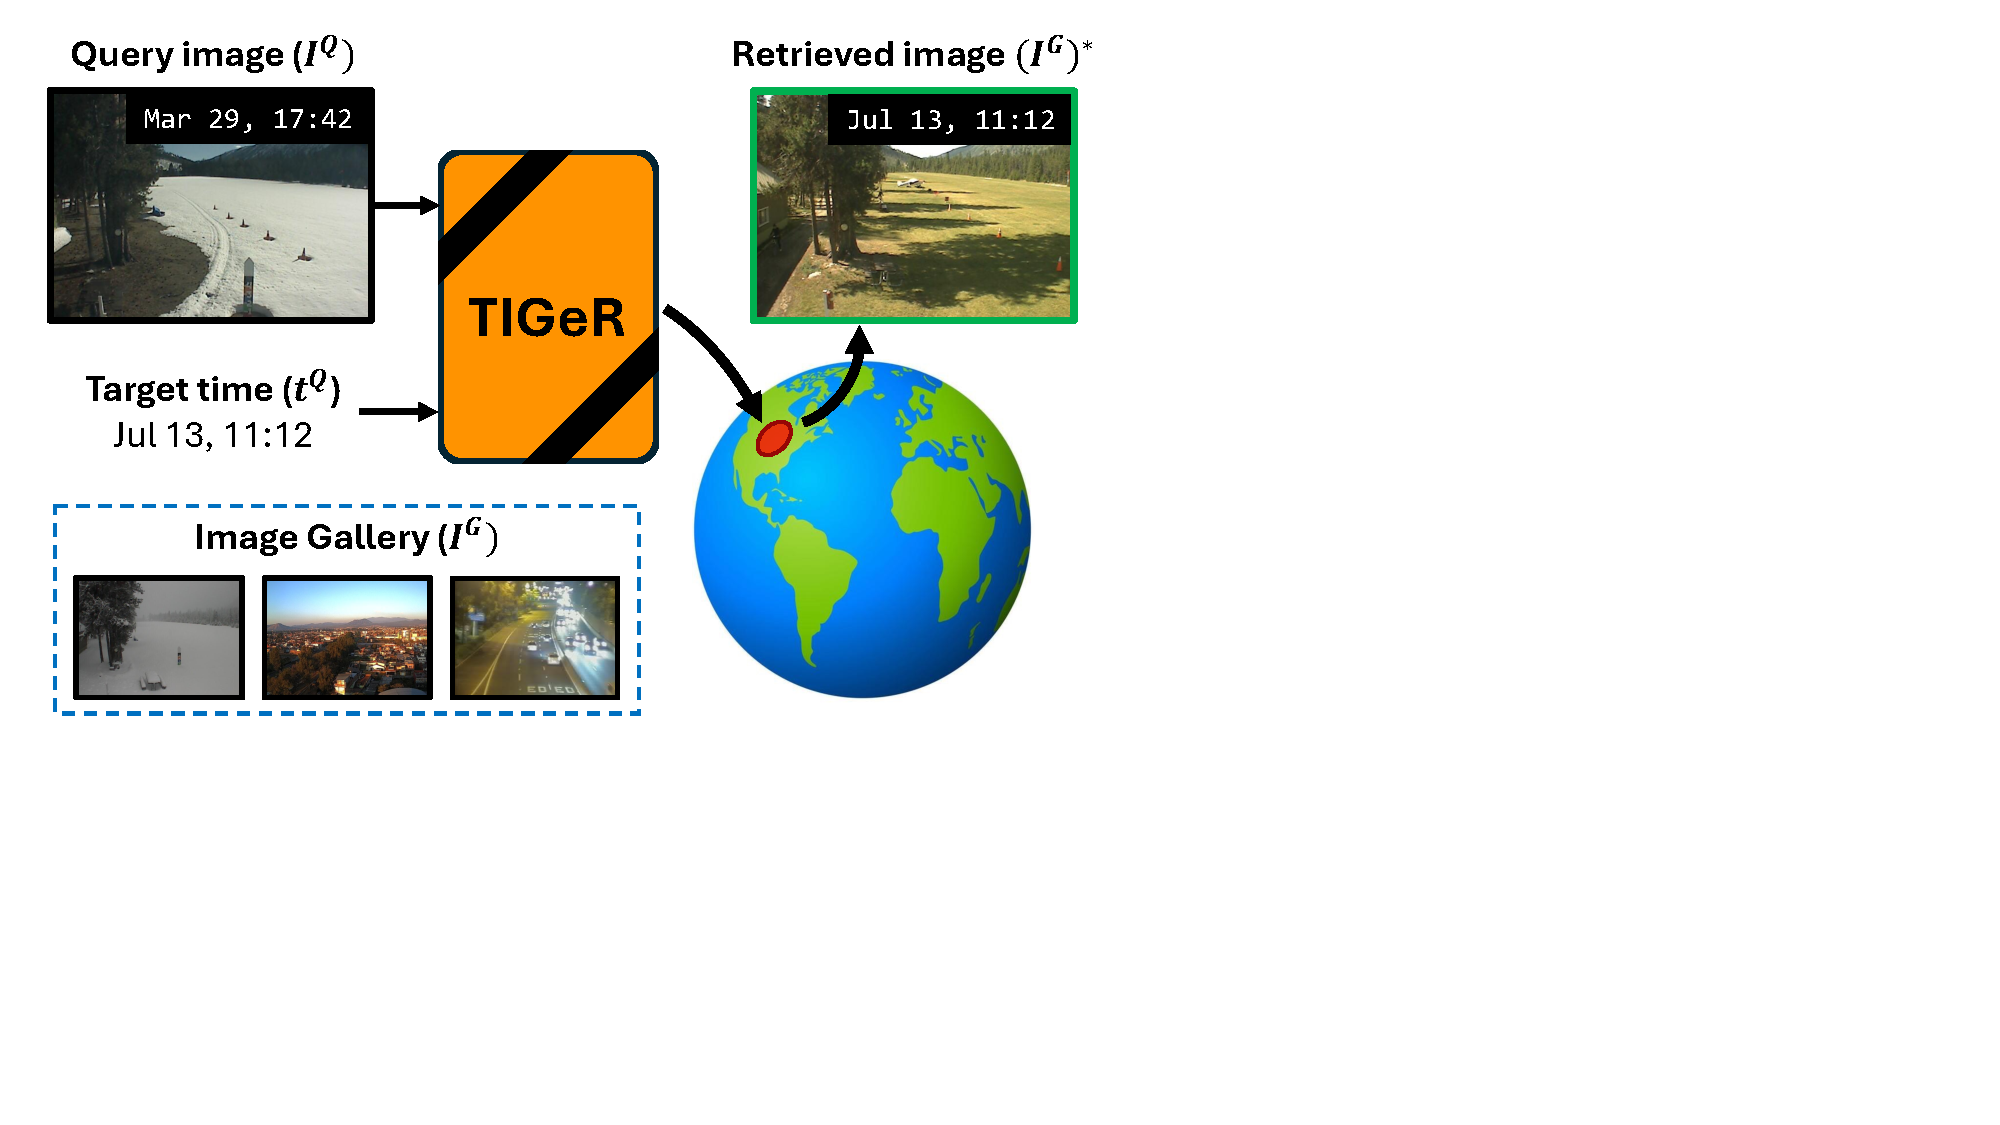
\includegraphics[width=0.9\linewidth]{figures/geotime-fig.pdf}
% \end{center}
% \vspace{-1em}
% \caption{\textbf{Schematic diagram of the geo-time-aware image retrieval task}. Given a query image $I^Q$ and a target time $t^Q$, the model retrieves a gallery image $I^G$ from (approximately) the same geographic location but matching the specified time.}
% \label{fig:geotime-fig}
% \end{figure}

We further analyze geo-time aware retrieval by comparing performance across the northern and southern hemispheres on \textsc{TIGeR-test-86k} and CVT.  
For every model and dataset, we compute Recall@10 separately for the northern (N-R@10) and southern (S-R@10) hemispheres, and report their ratio (N/S). 
Ratios closer to 1 indicate more balanced performance between hemispheres. 
As shown in Table~\ref{tab:geotime-hemispheres}, \tiger not only achieves the highest recall on both datasets, but also exhibits the most balanced N/S ratios, indicating the most geographically robust retrieval.

\begin{table}[h!]
\centering
\caption{\textbf{Hemispheric balance in geo-time-aware image retrieval.} 
We report Recall@10 on the northern (N-R@10) and southern (S-R@10) hemispheres, along with their ratio (N/S), for \textsc{TIGeR-test-86k} and CVT. 
Values of N/S closer to 1 indicate more balanced performance across hemispheres. 
\tiger attains both the highest recalls and the most balanced N/S ratios on both datasets.}
\label{tab:geotime-hemispheres}
\resizebox{\columnwidth}{!}{
\begin{tabular}{lcccccc}
\toprule
\multirow{2}{*}{\textbf{Method}} 
& \multicolumn{3}{c}{\textbf{TIGeR-Test-86k}} 
& \multicolumn{3}{c}{\textbf{CVT}} \\
\cmidrule(lr){2-4} \cmidrule(lr){5-7}
& \textbf{N-R@10} & \textbf{S-R@10} & \textbf{N/S}
& \textbf{N-R@10} & \textbf{S-R@10} & \textbf{N/S} \\
\midrule
Zhai et al.        & 8.47  & 14.12 & 0.60 & 3.35  & 1.46  & 2.29 \\
Zhai et al. CLIP   & 11.43 & 16.07 & 0.71 & 17.09 & 9.86  & 1.73 \\
GT-Loc             & 2.46  & 3.47  & 0.71 & 27.26 & 17.92 & 1.52 \\
\midrule
\textbf{TIGeR}     & \textbf{32.15} & \textbf{43.13} & \textbf{0.75} 
                   & \textbf{33.73} & \textbf{26.46} & \textbf{1.27} \\
\bottomrule
\end{tabular}
}
\end{table}



\section{Analysis on time prediction}
\label{sup:time-pred}

In Figure \ref{fig:conf-mats}, we present the confusion matrices comparing \tiger and GT-Loc on both \textsc{TIGeR-test-86k} and CVT to evaluate the quality of our time-of-year (ToY) and time-of-day (ToD) predictions. A perfect temporal predictor produces a strictly diagonal confusion matrix, indicating that predicted time bins match the ground truth exactly.

Across both benchmarks, \tiger exhibits sharp, well-defined diagonals in both ToY and ToD matrices, with only small amounts of spread into adjacent bins. This pattern reflects precise temporal reasoning: predictions are correct or fall within the nearest neighboring month or hour, consistent with natural continuity in seasonal and lighting conditions.
In contrast, GT-Loc produces more off-diagonal mass, with predictions often drifting toward a narrow range of time bins, especially in the ToD setting. This indicates difficulty in capturing fine-grained temporal cues and a tendency to over-smooth predictions toward frequent modes.
Overall, the confusion matrices clearly show that \tiger delivers substantially stronger temporal predictions, maintaining tight alignment between predicted and true time bins and demonstrating markedly improved geo-temporal understanding compared to GT-Loc.

\begin{figure*}[h]
\begin{center}
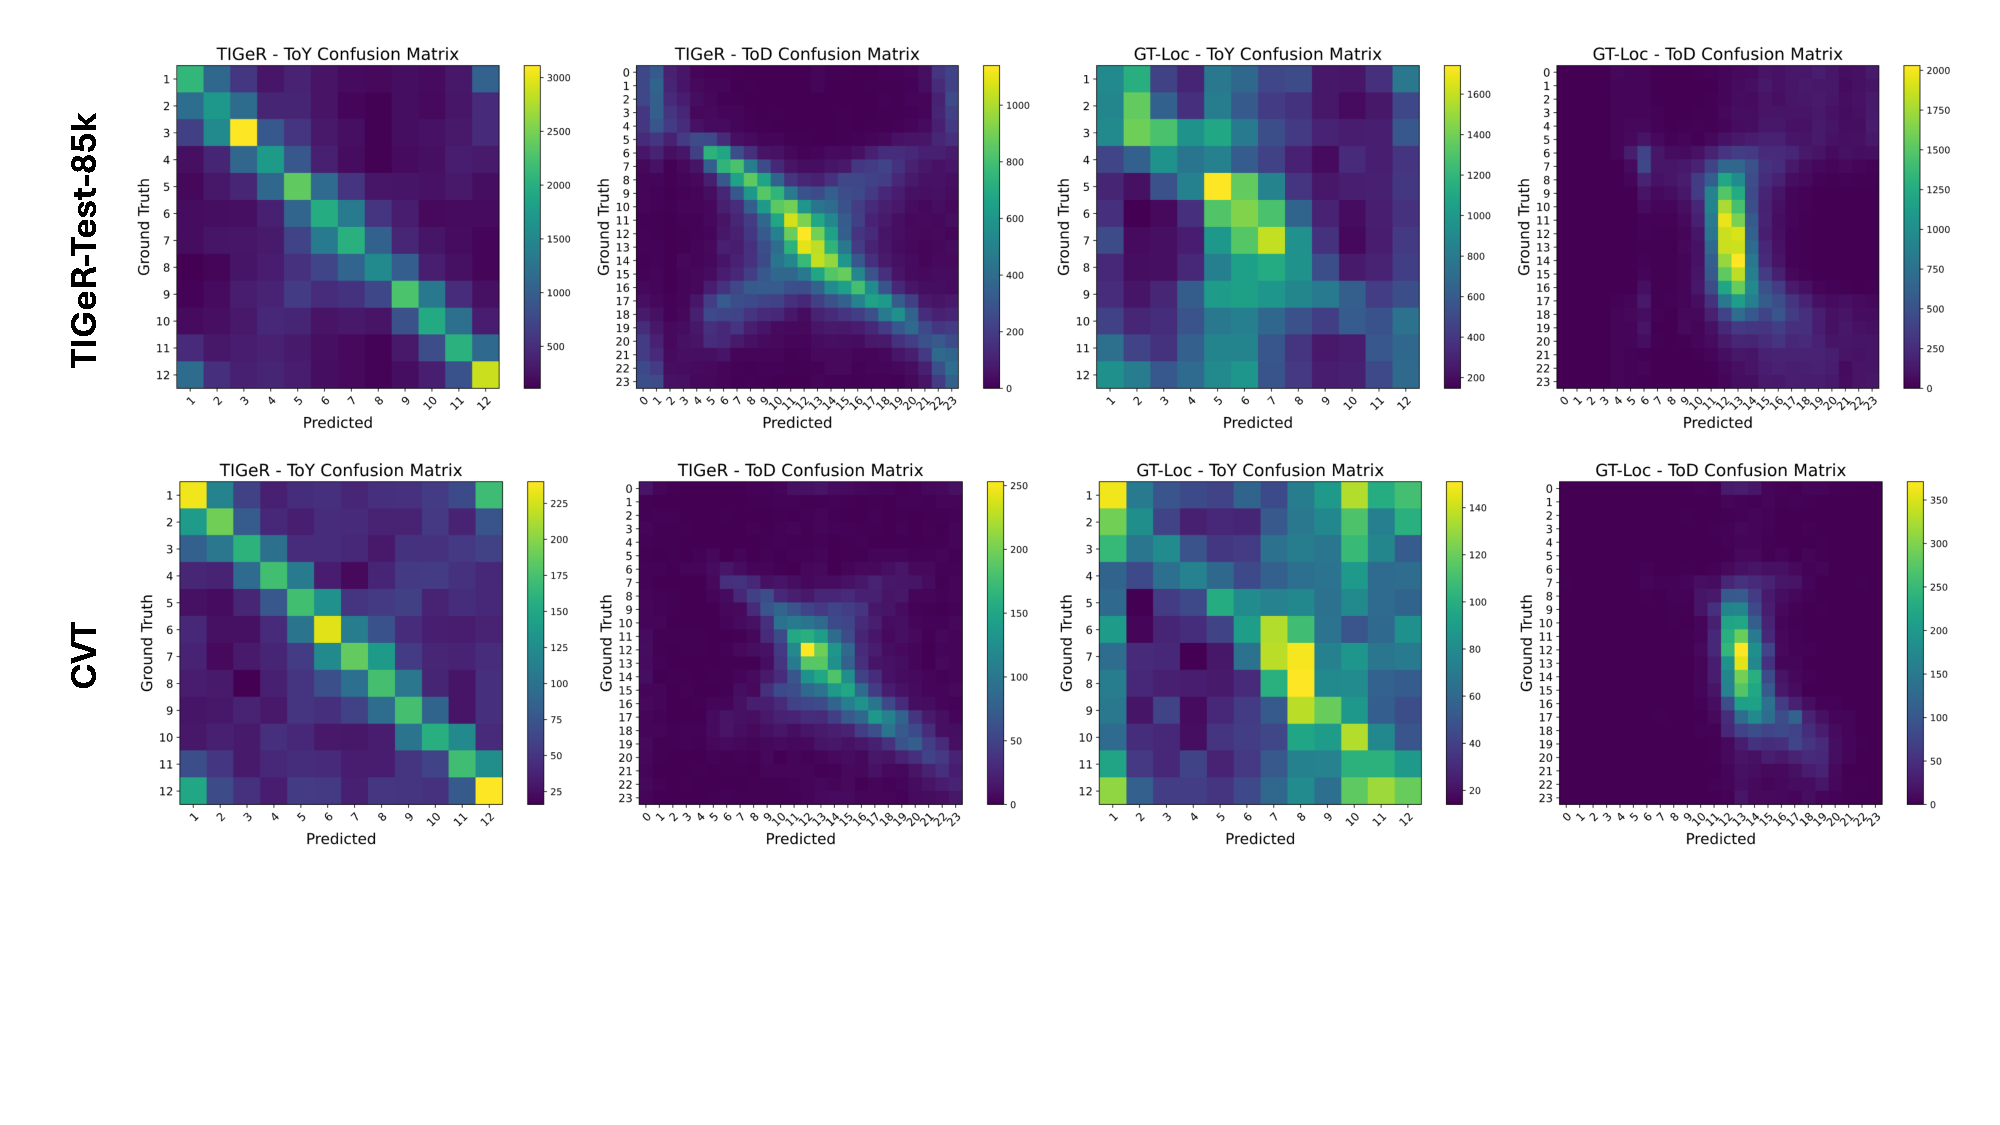
\includegraphics[width=0.9\linewidth]{figures/conf_mats.pdf}
\end{center}
\vspace{-1em}
\caption{\textbf{Confusion matrices} for \tiger and GT-Loc \cite{Shatwell_2025_ICCV} on the \textsc{TIGeR-test-86k} and CVT benchmarks. Ground-truth and predicted time-of-year (ToY) and time-of-day (ToD) are discretized into 12 monthly bins and 24 hourly bins, respectively. \tiger exhibits strong diagonal structure in both ToY and ToD matrices, indicating that predictions closely match the ground truth, with most errors occurring in adjacent temporal classes. This highlights \tiger’s substantially superior temporal-prediction performance compared to GT-Loc.
}
\label{fig:conf-mats}
\end{figure*}







\section{Additional time-prediction baselines}

TICL~\cite{lin2025what} is a recent image–time pretraining approach that leverages contrastive learning to align image and temporal embeddings within a shared feature space, similar in spirit to GeoCLIP~\cite{vivanco2024geoclip} and GT-Loc~\cite{Shatwell_2025_ICCV}. The resulting pretrained model can be applied to downstream tasks such as time-based image retrieval, video scene classification, and time-aware image editing, demonstrating the benefits of temporally aware representations. For a fair comparison, we train TICL for joint time-of-year (ToY) and time-of-day (ToD) prediction on our proposed dataset, closely following the original training protocol. As shown in Table~\ref{tab:ticl-baseline}, TIGeR consistently achieves lower time prediction errors across all metrics on both the \textsc{TIGeR-test-86k} and CVT test sets, further supporting the conclusion that jointly modeling geo-location and time with early fusion yields more effective temporal representations.

\begin{table}[t]
\centering
\setlength{\aboverulesep}{0pt}
\setlength{\belowrulesep}{0pt}
\caption{\textbf{Time prediction with additional baselines}. We train and test TICL~\cite{lin2025what} on our proposed dataset, closely adhering to the training protocol outlined by the authors.}
\label{tab:ticl-baseline}
\begingroup
\setlength{\tabcolsep}{1pt}
\resizebox{\linewidth}{!}{
\begin{tabular}{lccccc} 
\toprule
\multirow{3}{*}{\textbf{Method}} & \multirow{3}{*}{\textbf{Retrieval}}
  & \multicolumn{2}{c}{\textbf{TIGeR-test-86k}}
  & \multicolumn{2}{c}{\textbf{CVT-test}} \\
\cmidrule(lr){3-4} \cmidrule(lr){5-6}
                & 
  & \textbf{ToY} & \textbf{ToD} 
  & \textbf{ToY} & \textbf{ToD}  \\
                & 
  & \textbf{Error}$\downarrow$ & \textbf{Error}$\downarrow$
  & \textbf{Error}$\downarrow$ & \textbf{Error}$\downarrow$  \\
\midrule

Zhai et al.~\cite{zhai2019learning}*                & $I \rightarrow t$ & 68.38 & 3.97 & 87.37 & 3.28  \\
Zhai et al. w/ CLIP ~\cite{zhai2019learning}*        & $I \rightarrow t$ & 57.51 & 3.22 & 68.95 & 2.8  \\
Time-Loc~\cite{Shatwell_2025_ICCV}*   & $I \rightarrow t$ & 74.87 & 4.02 & 65.10 & 2.86 \\
GT-Loc~\cite{Shatwell_2025_ICCV}*    & $I \rightarrow t$  & 74.58 & 3.52 & 78.95 & \textbf{2.68} \\
TICL~\cite{lin2025what}* & $I \rightarrow t$  & 59.88 & 3.47 & 72.63 & 3.27 \\

\midrule

\textbf{TIGeR (Ours)}    & $I \rightarrow t$  & \textbf{51.49} & \textbf{3.13} & \textbf{62.88} & 2.73 \\

\bottomrule
\end{tabular}}
\endgroup
\end{table}



\section{Training details}
\label{sup:training-details}

\paragraph{Optimization and schedule.}
We train TIGeR for 10k iterations with a global batch size of 1024. 
Validation on all benchmarks is performed every 500 iterations, corresponding to 20 training epochs over the effective number of iterations.
We use the AdamW optimizer with $(\beta_1,\beta_2) = (0.9, 0.999)$ and weight decay $10^{-3}$.
The learning rate follows a cosine decay schedule from a maximum value of $10^{-4}$ down to $10^{-7}$, with a linear warm-up phase during the first 100 iterations.
All experiments are run on a single NVIDIA H100 GPU with 80\,GB of memory, 88\,GB of system RAM, and a 12-core CPU.

\vspace{-1em}
\paragraph{Image encoder and augmentations.}
The image branch uses a pretrained ViT-L/14 CLIP encoder \cite{clip}, which is kept frozen during training and only serves to extract visual tokens as described in Section~4 of the main paper.
Input images are pre-processed with a standard CLIP-style pipeline.
Concretely, we apply a random resized crop to size $224\times224$ with scale sampled from $[0.6, 1.0]$ and aspect ratio from $[0.9, 1.1]$ using bicubic interpolation. 
We then convert the image to RGB, and with probability $0.25$ apply a mild color jitter (brightness, contrast, and saturation each sampled from $[-0.1, 0.1]$).
A random horizontal flip is applied with probability $0.5$.
Finally, images are converted to tensors and normalized with the mean and standard deviation used by CLIP.

\vspace{-1em}
\paragraph{Location and time encoders.}
Location and time are encoded with random Fourier feature (RFF) encoders, each followed by a small MLP.
GPS coordinates and temporal coordinates are first mapped from $\mathbb{R}^2$ into a 1024-dimensional feature space using a bank of sinusoidal projections with frequencies $\{2^0, 2^1, \dots, 2^9\}$.
The resulting RFF features are passed through a modality-specific MLP and layer normalization to produce the token sequences $L$ and $T$ used by the multimodal transformer.

\vspace{-1em}
\paragraph{Fusion transformer.}
The shared fusion module $\mathcal{F}(\cdot)$ is implemented as a single Transformer block that operates jointly on the concatenated tokens from the active modalities (image, location, and/or time).
The block uses 64 attention heads and the same hidden dimension as the encoder outputs (1024), and is shared across all six input configurations (single-modality and pair-wise modality inputs), as detailed in Section~4 of the main paper.
We found that a single well-parameterized block is sufficient to capture useful cross-modal interactions while keeping training efficient.

\begin{figure*}[t]
\begin{center}
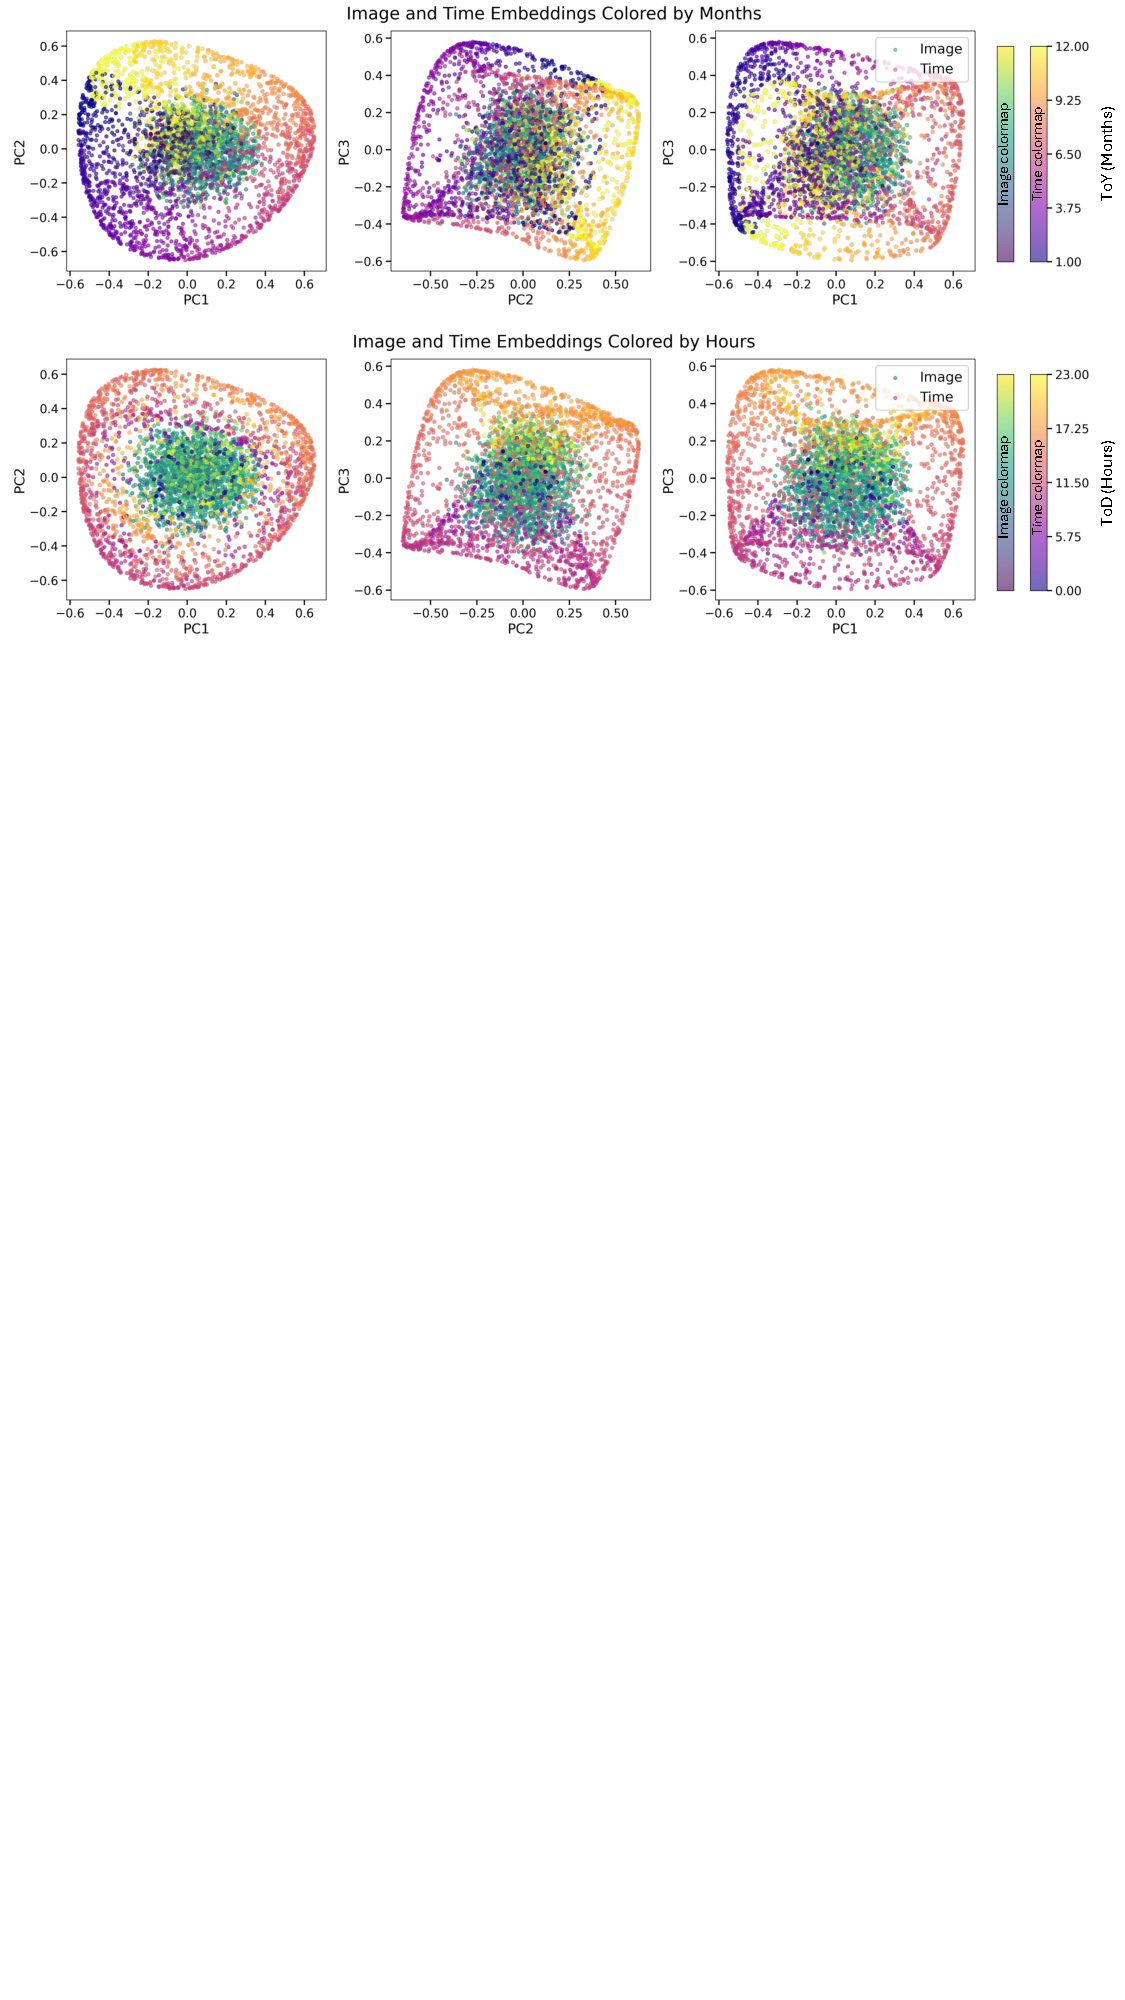
\includegraphics[width=0.8\linewidth]{figures/pca.pdf}
\end{center}
\vspace{-1em}
\caption{\textbf{PCA visualization of the \tiger\ embedding space.}
We project 2{,}000 image--timestamp pairs from the CVT test set onto the first three principal components computed from the time embeddings, and apply the same projection to the corresponding image embeddings.
\textbf{Top:} embeddings colored by time-of-year (month). 
\textbf{Bottom:} embeddings colored by time-of-day (hour). 
Image embeddings (green--yellow) follow the toroidal structure traced by the time embeddings (purple--orange), showing that \tiger\ aligns visual and temporal features on a shared, torus-like manifold.
}
\label{fig:pca_supp}
\end{figure*}

\vspace{-1em}
\paragraph{Metric-aware classification heads.}
For geo-location classification, we discretize the Earth into HEALPix cells with $\text{NSIDE}=8$, yielding 768 equal-area regions.
For each training sample we compute the corresponding cell index and use the cell center as the class prototype.
Soft labels are constructed using the metric-affinity formulation from Eq.~(5) in the main paper, with Haversine distance as the metric and temperature $\gamma_{\text{geo}} = 250$.
For time, we discretize the flat torus $\mathbb{T}^2$ into $24\times 12 = 288$ bins corresponding to one-hour (ToD) and one-month (ToY) intervals.
Temporal soft labels are obtained using the torus geodesic distance with temperature $\gamma_{\text{time}} = 1$.
In both cases, a two-layer MLP applied to the pooled image embedding produces logits over the corresponding class space, which are trained with cross-entropy against the soft metric targets.

\vspace{-1em}
\paragraph{Training data and supervision.}
The main training signal comes from \textsc{TIGeR-Train-4.5M} and CVT, both of which provide image, geo-location, and timestamp annotations.
These datasets are used to optimize all components: contrastive losses over the unified embedding space, the multimodal fusion transformer, and the metric-aware classification heads.
In addition, we leverage auxiliary datasets that provide only images and location data (e.g., Google Landmarks v2 \cite{weyand2020google}, MP-16 \cite{7849098}, and OpenStreetViews 5M \cite{astruc2024openstreetview}).
For these datasets, we only train compute the loss using the image-location contrastive and classification losses using the same metric-aware targets.

\vspace{-1em}
\paragraph{Batch construction and debiasing.}
Some of the underlying datasets exhibit strong geographic imbalance, with a heavy skew toward North America and Europe.
To mitigate this, we enforce diversity at the batch level.
Each training batch of size 1024 is constructed by first sampling at least 64 distinct HEALPix cells at $\text{NSIDE}=8$.
For each selected cell, we then sample up to 16 images whose GPS coordinates fall inside that cell.
Whenever possible, we also enforce temporal diversity within each cell by avoiding repeated month--hour combinations; i.e., we try not to include two samples in the same batch that share the same (ToY, ToD) pair among the 288 possible configurations.
This strategy yields batches that are both geographically and temporally diverse, improving robustness and preventing the model from overfitting to overrepresented regions.

\vspace{-1em}
\paragraph{Entropy-adaptive reranking.}
At test time, we apply the entropy-adaptive reranking scheme described in Eqs.~(8)--(9) of the main paper to combine continuous retrieval scores with the classifier-based priors for geo-location and time.
For location retrieval, we use a similarity temperature $\psi_{\text{geo}} = 0.07$ and a maximum prior weight $\beta_{\text{geo}}^{\max} = 1$.
For time prediction, we set $\psi_{\text{time}} = 0.07$ and $\beta_{\text{time}}^{\max} = 2$.
The actual prior weight $\beta(I^Q)$ for a query image $I^Q$ is modulated by the entropy of the predicted class distribution, so that confident predictions rely more strongly on the prior, while uncertain ones fall back on pure similarity-based retrieval.

\vspace{-1em}
\paragraph{Baseline reproducibility.}
All baselines are reproduced as closely as possible by following the training details provided in their respective papers. For a fair comparison with our method, we train all baselines on the \textsc{TIGeR-test-86k} and CVT datasets. In the baseline variants where the original CNN backbone is replaced with a pretrained CLIP ViT, we also match the number of gradient updates used by our method to ensure a consistent and fair comparison.

\section{Embedding space visualization}
\label{sup:embedding}

To inspect the structure of the learned geo-temporal representation, we visualize a PCA projection of the joint embedding space (Figure \ref{fig:pca_supp}). We randomly sample 2{,}000 image-time pairs from the CVT test set and compute PCA on the time embeddings; the resulting projection is then applied to the corresponding image embeddings so that both modalities share the same principal-component basis. Image embeddings are shown with a green--yellow colormap, and time embeddings with a purple--orange colormap. We display the three pairwise combinations of the first three components (PC1--PC2, PC2--PC3, and PC1--PC3) to better reveal the global geometry of the space.

The top row colors each point by time-of-year (month). Both image and time embeddings trace a smooth circular pattern along the outer ring, with neighboring months occupying adjacent regions. The bottom row colors points by time-of-day (hour), revealing a complementary cycle that wraps around an inner ring. Taken together, these views indicate that \tiger organizes image and time features on a low-dimensional, torus-like manifold, consistent with our design choice of encoding time as a point on the flat torus~$\mathbb{T}^2$.


